%In 2013, a report by the U.S. National Climate Assessment provided evidence that the most recent decade was the nation's warmest on record~\cite{melillo2014climate} and experts predict that temperatures are only going to rise.


2015 was the hottest year on record since the beginning of weather recording in 1880~\cite{noaa}. 
Heat waves in summer and polar vortexes in winter are growing longer and pose increasing challenges to an already over-stressed electric grid. 
Furthermore, with the increasing penetration of renewable generation, the electricity grid is also experiencing a shift from predictable and dispatchable electricity generation to variable and non-dispatchable generation. 
This adds another level of uncertainty and volatility to the electricity grid.
The volatility due to the mismatch between electricity generation and supply further leads to volatility in the wholesale price of electricity.
For \eg the polar vortex triggered extreme weather events in the U.S. in January 2014, which caused many electricity customers to experience increased costs.
Parts of the U.S. north-eastern electricity grid experienced a 86 fold increase in the price of electricity from $\$31/\si{\mega\watt\hour}$ to $\$2,680/\si{\mega\watt\hour}$ in a matter of a few minutes~\cite{volatility}. 
%Similarly, the summer price spiked $32$ fold from an average of $\$25/\si{\mega\watt\hour}$ to $\$800/\si{\mega\watt\hour}$ in July of 2015.
Such events show how unforeseen and uncontrollable circumstances can greatly affect electricity prices that impact grid operator and customers. 
%Energy industry experts are now considering the concept that extreme weather, more renewables and resulting 
Electricity price volatility, is becoming the new norm rather than the exception.

Across the United States, utilities and grid operators are devoting increasing attention and resources to demand response (DR). It is considered as a reliable means of mitigating the uncertainty and volatility of renewable generation and extreme weather conditions and improving the grid's efficiency and reliability.
The resource contribution from all U.S. demand response programs is estimated to be nearly 72,000 MW, or about 9.2 percent of U.S. peak demand~\cite{federal2008assessment} making DR the largest virtual generator in the U.S. national grid.
The annual revenue to end-users from DR markets with PJM ISO alone is more than \$700 million~\cite{pjm}. 
Global DR revenue is expected to reach nearly \$40 billion from 2014 through 2023~\cite{navigant}.

%\begin{figure}
%\centering
%\includegraphics[width=\columnwidth]{figs/twocolumnnew-compressed}
%\caption{Majority of DR today is manual and rule-based. (a) The fixed rule based DR is inconsistent and could under-perform compared to the required curtailment, resulting in DR penalties. (b) Using data-driven models DR-Advisor uses DR strategy evaluation and DR strategy synthesis for a sustained and sufficient curtailment.}
%\label{fig:twocolumn}
%\vspace{-10pt}
%\end{figure}

The volatility in real-time electricity prices poses the biggest operational and financial risk for large scale end-users of electricity such as large commercial buildings, industries and institutions; often referred to as \textit{C/I/I} consumers. 
In order to shield themselves from the volatility and risk of high prices, such consumers must be more flexible in their electricity demand. 
Consequently, large \textit{C/I/I} customers are increasingly looking to demand response programs to help manage their electricity costs.
DR programs involve a voluntary response of a building to a price signal or a load curtailment request from the utility or the curtailment service provider (CSP). 
Upon successfully meeting the required curtailment level the end-users are financially rewarded, but may also incur penalties for under-performing and not meeting a required level of load curtailment.
In practice, one of the biggest challenges with end-user demand response is the following: \emph{Upon receiving the notification for a DR event, what actions must the end-user take in order to achieve an adequate and a sustained DR curtailment?} 

This is a hard question to answer because of the following reasons:
\begin{enumerate}[leftmargin=0.5cm,topsep=1pt,itemsep=-1ex,partopsep=1ex,parsep=1ex]
\item \textbf{Modeling complexity and heterogeneity}: Unlike the automobile or the aircraft industry, each building is designed and used in a different way and therefore, it must be uniquely modeled. 
Learning predictive models of building's dynamics using first principles based approaches (\eg with EnergyPlus~\cite{Crawley2001319}) is very cost and time prohibitive and requires retrofitting the building with several sensors~\cite{costmpc};
The user expertise, time, and associated sensor costs required to develop a model of a single building is very high.
%This is because usually a building modeling domain expert typically uses a software tool to create the geometry of a building from the building design and equipment layout plans, add detailed information about material properties, about equipment and operational schedules. 
%There is always a gap between the modeled and the real building and the domain expert must then manually tune the model to match the measured data from the building~\cite{new2012autotune}. 
\item \textbf{Limitations of rule-based DR}: The building's operating conditions, internal thermal disturbances and environmental conditions must all be taken into account to make appropriate DR control decisions, which is not possible with using rule-based and pre-determined DR strategies since they do not account for the state of the building but are instead based on best practices and rules of thumb. 
%As shown in Fig.~\ref{fig:twocolumn}(a), the performance of a rule-based DR strategy is inconsistent and can lead to reduced amount of curtailment which could result in penalties to the end-user. 
%In our work, we show how a data-driven DR algorithm outperforms a rule-based strategy by $17\%$ while accounting for thermal comfort.
Rule based DR strategies have the advantage of being simple but they do not account for the state of the building and weather conditions during a DR event.
%Despite this lack of predictability, rule-based DR strategies account for the majority of DR approaches.
\item \textbf{Control complexity and scalability}: Upon receiving a notification for a DR event, the building's facilities manager must determine an appropriate DR strategy to achieve the required load curtailment. 
These control strategies can include adjusting zone temperature set-points, supply air temperature and chilled water temperature set-point, dimming or turning off lights, decreasing duct static pressure set-points and restricting the supply fan operation \etc. 
In a large building, it is difficult to assess the effect of one control action on other sub-systems and on the building's overall power consumption because the building sub-systems are tightly coupled. 
%Consider the case of the University of Pennsylvania's campus, which has over a hundred different buildings and centralized chiller plants. In order to perform campus wide DR, the facilities manager must account for several hundred thousand set-points and their impact on the different buildings. Therefore, it is extremely difficult for a human operator to accurately gauge the building's or a campus's response.
\item \textbf{Interpretability of modeling and control}: Predictive models for buildings, regardless how sophisticated, lose their effectiveness unless they can be interpreted by human experts and facilities managers in the field.
%For \eg artificial neural networks (ANN) obscure physical control knobs and interactions and hence, are difficult to interpret by building facilities managers.
Therefore, the required solution must be transparent, human centric and highly interpretable.
\end{enumerate}

\begin{figure}
\centering
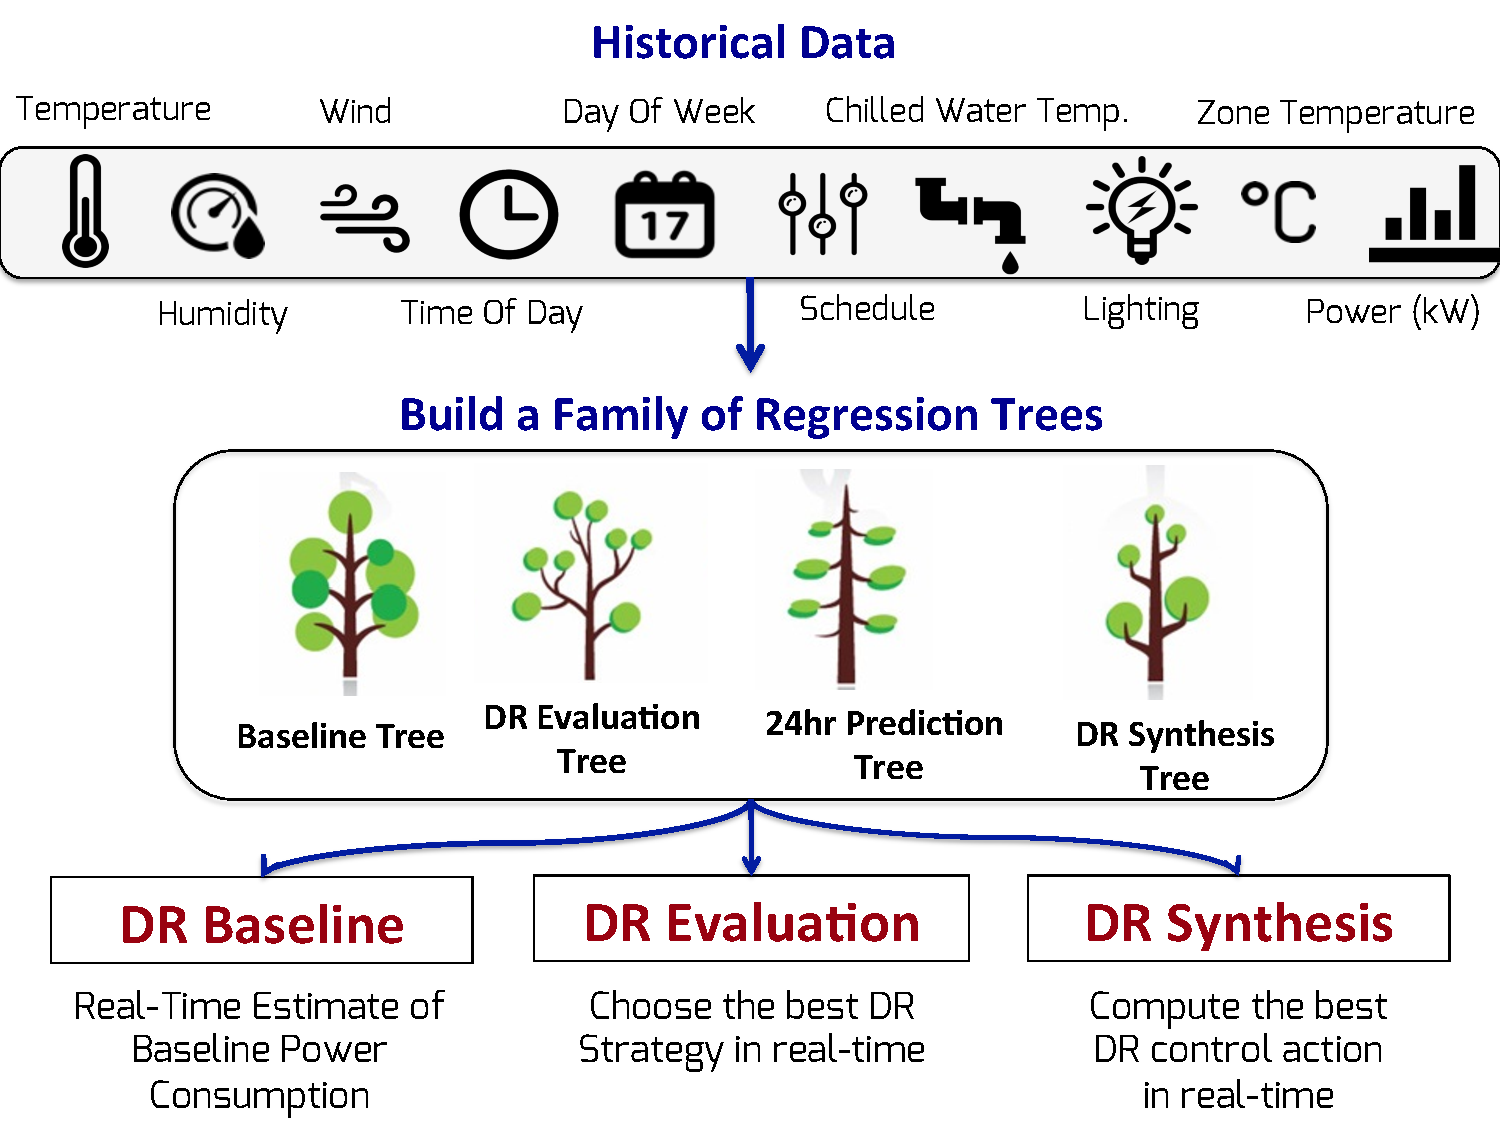
\includegraphics[width=0.6\columnwidth]{figs/overview.pdf}
\caption{Overview of DR-Advisor Architecture.}
\label{fig:overview}
\end{figure}

The goal with data-driven methods for cyber-physical energy systems is to make the best of both worlds; i.e. simplicity of rule based approaches and the predictive capability of model based strategies, but without the expense of first principle or grey-box model development.

In this paper, we present a method called DR-Advisor (Demand Response-Advisor), which acts as a recommender system for the building's facilities manager and provides the power consumption prediction and control actions for meeting the required load curtailment and maximizing the economic reward.  
Using historical meter and weather data along with set-point and schedule information, DR-Advisor builds a family of interpretable regression trees to learn non-parametric data-driven models for predicting the power consumption of the building (Fig.~\ref{fig:overview}).
DR-Advisor can be used for real-time demand response baseline prediction, strategy evaluation and control synthesis, without having to learn first principles based models of the building.
We build on our previous work on data-driven demand response~\cite{BehlJainMangharam2016} and present a receding horizon predictive control algorithm for demand response and peak power reduction. 

\subsection{Contributions}

This work has the following data-driven contributions:

\begin{enumerate}
\item \textbf{Demand Response:}
\begin{enumerate} %[leftmargin=0.5cm,topsep=1pt,itemsep=-1ex,partopsep=1ex,parsep=1ex]
\item \textbf{Baseline Prediction:} We demonstrate the benefit of using regression trees based approaches for estimating the demand response baseline power consumption. Using regression tree-based algorithms eliminates the cost of time and effort required to build and tune first principles based models of buildings for DR. 
DR-Advisor achieves a prediction accuracy of 92.8\% to 98.9\% for baseline estimates of eight buildings on the Penn campus.
\item \textbf{Strategy Evaluation:} We present an approach for building auto-regressive trees and apply it for demand response strategy evaluation. 
%Our models takes into account the state of the building and weather forecasts to help choose the best DR strategy among several pre-determined strategies.
\item \textbf{Control Synthesis:}  We introduce a novel model based control with regression trees (mbCRT) algorithm to enable control with regression trees and use it for real-time DR synthesis. Using the mbCRT algorithm, we can optimally trade off thermal comfort inside the building against the amount of load curtailment. While regression trees are a popular choice for prediction based models, this is the first time regression tree based algorithms have been used for controller synthesis with applications in demand response. Our synthesis algorithm outperforms rule based DR strategy by 17\% while maintaining bounds on thermal comfort inside the building.
\end{enumerate}

\item \textbf{Peak Power Reduction:}
\begin{enumerate} %[leftmargin=0.5cm,topsep=1pt,itemsep=-1ex,partopsep=1ex,parsep=1ex]
\item \textbf{Multi-variate output regression trees:} We also present a method for constructing a multi-variate output predictive model using regression trees. This is done by modifying the variable selection and splitting criteria at the nodes of the regression tree.
% The proposed algorithm achieves an accuracy of 90\% on test data set.
\item \textbf{Data predictive control:} We extend the mbCRT algorithm and present a data predictive control with regression trees (DPCRT) algorithm for finite receding horizon control. The algorithm is applied for peak power curtailment on a large office building, we evaluations show that DPCRT outperforms mbCRT by 8.6\%.
\end{enumerate}

We evaluate the performance of DR-Advisor using a mix of real data from 8 buildings on the campus of the University of Pennsylvania, in Philadelphia, USA and data-sets from a virtual building test-bed for the Department of Energy's (DoE) large commercial reference building. We also compare the performance of DR-Advisor against other data-driven methods using a bench-marking data-set from AHRAE's great energy predictor shootout challenge.
%The DPCRT algorithm is first of its kind that does finite receding horizon control with regression trees. 
%We evaluate the performance of our methods using a U.S. Department of Energy (DoE) commercial reference building model.
The data predictive control methods presented in this paper bypass the cost and time prohibitive process of building high fidelity models of buildings that use grey and white box modeling approaches while still being suitable for receding horizon control design.
These are the first algorithms of its kind that enable closed loop control synthesis and  finite receding horizon control with regression trees. 

\end{enumerate}

This paper is organized as follows. Sec.~\ref{sec:problem} describes the demand response problem. 
In Sec.~\ref{sec:drtree}, we present how data-driven algorithms can be used for the problems associated with DR. 
Sec.~\ref{sec:drsyn} presents a new algorithm to perform control with regression trees for synthesizing demand response strategies.
In Sec.~\ref{S:decision_tree}, a multi-variate output regression tree algorithm is presented. The receding horizon data-predictive control algorithm is described in Sec.~\ref{S:control_tree}.
Sec.~\ref{sec:case} presents a comprehensive case study using data from 8 real buildings and a virtual test-bed.
In Sec.~\ref{sec:related}, a short survey of related work has been presented. 
We conclude this paper in Sec.~\ref{sec:discussion} with a summary of the results. 
%and a discussion about future directions.